% !TEX TS-program = pdflatex
% !TEX encoding = UTF-8 Unicode

\documentclass[12pt]{article} 

\usepackage[utf8]{inputenc} % set input encoding 
\usepackage{geometry} % to change the page dimensions
\geometry{a4paper} 
\usepackage[parfill]{parskip} % No indent in document

% Packages
\usepackage{graphicx}
\usepackage{array}
\usepackage{amsmath}
\usepackage{amssymb}
\usepackage{verbatim}
\usepackage{xcolor}
\usepackage[hidelinks]{hyperref}
\usepackage{tikz}

\usepackage{todonotes}
\setuptodonotes{inline, size=\small}


% Define colors
\definecolor{mint}{rgb}{0.65,0.84,0.82}
\definecolor{scheme}{rgb}{0,0,1}

\title{Bitcoin, Blockchain and Cryptoassets \\ Solutions Exercise Set 2}
\author{}
\date{} 

\begin{document}
	\maketitle
	
	\newpage
	\section*{Exercise 1}
	As a quick reminder, here are the three protocol-based fork types presented in the lecture.
	
	\begin{figure}[h!]
		\centering
		\begin{minipage}{0.3\textwidth}
			\centering
			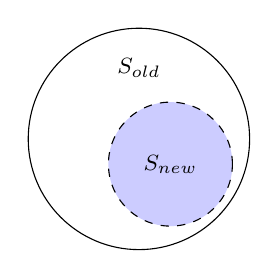
\begin{tikzpicture}[domain=0:8, scale=0.8]
				\filldraw[draw=black,fill=white] (0,0) circle (50pt) node[below=-1.15cm,color=black]{\footnotesize{$S_{old}$}};
				\filldraw[draw=black,fill=scheme!20,dashed] (0.5,-0.4) circle (28pt) node[color=black]{\footnotesize{$S_{new}$}};
			\end{tikzpicture}
			\center
			\textbf{Soft fork}
		\end{minipage}
		\hfill
		\begin{minipage}{0.3\textwidth}
			\centering
			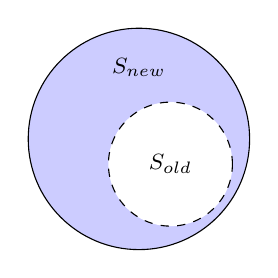
\begin{tikzpicture}[domain=0:8, scale=0.8]
				\filldraw[draw=black,fill=scheme!20] (0,0) circle (50pt) node[below=-1.15cm,color=black]{\footnotesize{$S_{new}$}};
				\filldraw[draw=black,fill=white,dashed] (0.5,-0.4) circle (28pt) node[color=black]{\footnotesize{$S_{old}$}};
			\end{tikzpicture}
			\center
			\textbf{Hard fork}
		\end{minipage}
		\hfill
		\begin{minipage}{0.3\textwidth}
			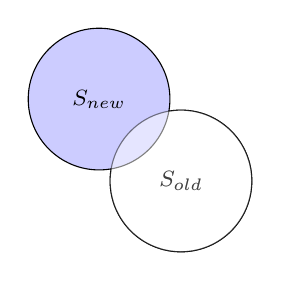
\begin{tikzpicture}[domain=0:8,scale=0.8, every node/.style={scale=1}]
				\filldraw[draw=black, fill=white] (0.9,-0.9) circle (32pt) node[color=black]{\footnotesize{$S_{old}$}};
				\filldraw[draw=black,fill=blue!20] (-0.4,0.4) circle (32pt) node[color=black]{\footnotesize{$S_{new}$}};
				\filldraw[draw=black, fill=white, opacity=0.5] (0.9,-0.9) circle (32pt) node[color=black]{\footnotesize{$S_{old}$}};
			\end{tikzpicture}
			\center
			\textbf{Forced fork}
		\end{minipage}
	\end{figure}
	
	We call a fork a soft fork if the new rules are more restrictive than the old ones ($S_{new}\subset S_{old}$). In a hard fork, the new rules are less restrictive than the old ones ($S_{new}\supset S_{old}$), and in a forced fork, no rule set completely includes the other rule set, but intersections are possible ($(S_{new}\setminus S_{old} \neq \emptyset)\wedge(S_{old}\setminus S_{new} \neq \emptyset)$). As you know from the lecture, miners will always continue mining at the longest chain, i.e. the chain that includes the most difficulty. The following table is useful to visualize the coming explanations.
	\vspace{0.5cm}
	\begin{table}[h!]
		\centering
		\resizebox{12cm}{!}{
			\begin{tabular}{ccc}
				\hline \hline
				& New dominant & Old dominant\\ \cline{2-3}
				&&\\
				Soft fork & 
				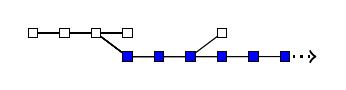
\begin{tikzpicture}[domain=1:10,scale=0.4, every node/.style={scale=0.4}]
					\coordinate (o1) at (1,1);
					\coordinate (o2) at (2,1);
					\coordinate (o3) at (3,1);
					\coordinate (o4) at (4,1);
					\coordinate (o5) at (5,1);
					\coordinate (o6) at (6,1);
					\coordinate (o7) at (7,1);
					\coordinate (o8) at (8,1);
					\coordinate (o9) at (9,1);
					\coordinate (o10) at (10,1);
					\coordinate (n1) at (1,0.25);
					\coordinate (n2) at (2,0.25);
					\coordinate (n3) at (3,0.25);
					\coordinate (n4) at (4,0.25);
					\coordinate (n5) at (5,0.25);
					\coordinate (n6) at (6,0.25);
					\coordinate (n7) at (7,0.25);
					\coordinate (n8) at (8,0.25);
					\coordinate (n9) at (9,0.25);
					\coordinate (n10) at (10,0.25);
					
					\draw[] (o1) to[] (o2);
					\draw[] (o1) to[] (o2) to[] (o3);
					\draw[] (o1) to[] (o2) to[] (o3) to[] (o4);
					\draw[] (o3) to[] (n4);
					\draw[] (o3) to[] (n4) to[] (n5);
					\draw[] (o3) to[] (n4) to[] (n5) to[] (n6);
					\draw[] (o3) to[] (n4) to[] (n5) to[] (n6) to[] (n7);
					\draw[] (o3) to[] (n4) to[] (n5) to[] (n6) to[] (n7) to[] (n8);
					\draw[] (o3) to[] (n4) to[] (n5) to[] (n6) to[] (n7) to[] (n8) to[] (n9);
					\draw[color=black] (n6) to[] (o7);
					\draw[color=black,thick, dotted, ->] (n9) to[] (n10);
					
					\node (rect) at (o1) [fill=white,draw,minimum width=0.3cm,minimum height=0.3cm] {};
					\node (rect) at (o2) [fill=white,draw,minimum width=0.3cm,minimum height=0.3cm] {};
					\node (rect) at (o3) [fill=white,draw,minimum width=0.3cm,minimum height=0.3cm] {};
					\node (rect) at (o4) [fill=white,draw,minimum width=0.3cm,minimum height=0.3cm] {};
					\node (rect) at (o7) [fill=white,draw,minimum width=0.3cm,minimum height=0.3cm] {};
					\node (rect) at (n4) [fill=scheme,draw,minimum width=0.3cm,minimum height=0.3cm] {};
					\node (rect) at (n5) [fill=scheme,draw,minimum width=0.3cm,minimum height=0.3cm] {};
					\node (rect) at (n6) [fill=scheme,draw,minimum width=0.3cm,minimum height=0.3cm] {};
					\node (rect) at (n7) [fill=scheme,draw,minimum width=0.3cm,minimum height=0.3cm] {};
					\node (rect) at (n8) [fill=scheme,draw,minimum width=0.3cm,minimum height=0.3cm] {};
					\node (rect) at (n9) [fill=scheme,draw,minimum width=0.3cm,minimum height=0.3cm] {};
				\end{tikzpicture} 
				&
				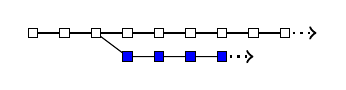
\begin{tikzpicture}[domain=1:10,scale=0.4, every node/.style={scale=0.4}]
					\coordinate (o1) at (1,1);
					\coordinate (o2) at (2,1);
					\coordinate (o3) at (3,1);
					\coordinate (o4) at (4,1);
					\coordinate (o5) at (5,1);
					\coordinate (o6) at (6,1);
					\coordinate (o7) at (7,1);
					\coordinate (o8) at (8,1);
					\coordinate (o9) at (9,1);
					\coordinate (o10) at (10,1);
					\coordinate (n1) at (1,0.25);
					\coordinate (n2) at (2,0.25);
					\coordinate (n3) at (3,0.25);
					\coordinate (n4) at (4,0.25);
					\coordinate (n5) at (5,0.25);
					\coordinate (n6) at (6,0.25);
					\coordinate (n7) at (7,0.25);
					\coordinate (n8) at (8,0.25);
					\coordinate (n9) at (9,0.25);
					\coordinate (n10) at (10,0.25);
					
					\draw[color=black] (o1) to[] (o2) to[] (o3) to[] (o4) to (o5) to (o6) to (o7) to (o8) to (o9);
					\draw[color=black] (o3) to[] (n4) to[] (n5) to[] (n6) to[] (n7);
					\draw[color=black,thick, dotted, ->] (o9) to[] (o10);
					\draw[color=black,thick, dotted, ->] (n7) to[] (n8);
					
					\node (rect) at (o1) [fill=white,draw,minimum width=0.3cm,minimum height=0.3cm] {};
					\node (rect) at (o2) [fill=white,draw,minimum width=0.3cm,minimum height=0.3cm] {};
					\node (rect) at (o3) [fill=white,draw,minimum width=0.3cm,minimum height=0.3cm] {};
					\node (rect) at (o4) [fill=white,draw,minimum width=0.3cm,minimum height=0.3cm] {};
					\node (rect) at (o5) [fill=white,draw,minimum width=0.3cm,minimum height=0.3cm] {};
					\node (rect) at (o6) [fill=white,draw,minimum width=0.3cm,minimum height=0.3cm] {};
					\node (rect) at (o7) [fill=white,draw,minimum width=0.3cm,minimum height=0.3cm] {};
					\node (rect) at (o8) [fill=white,draw,minimum width=0.3cm,minimum height=0.3cm] {};
					\node (rect) at (o9) [fill=white,draw,minimum width=0.3cm,minimum height=0.3cm] {};
					
					\node (rect) at (n4) [fill=scheme,draw,minimum width=0.3cm,minimum height=0.3cm] {};
					\node (rect) at (n5) [fill=scheme,draw,minimum width=0.3cm,minimum height=0.3cm] {};
					\node (rect) at (n6) [fill=scheme,draw,minimum width=0.3cm,minimum height=0.3cm] {};
					\node (rect) at (n7) [fill=scheme,draw,minimum width=0.3cm,minimum height=0.3cm] {};
					
				\end{tikzpicture}    
				\\
				&&\\
				Hard fork &
				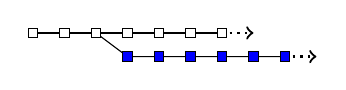
\begin{tikzpicture}[domain=1:10,scale=0.4, every node/.style={scale=0.4}]
					\coordinate (o1) at (1,1);
					\coordinate (o2) at (2,1);
					\coordinate (o3) at (3,1);
					\coordinate (o4) at (4,1);
					\coordinate (o5) at (5,1);
					\coordinate (o6) at (6,1);
					\coordinate (o7) at (7,1);
					\coordinate (o8) at (8,1);
					\coordinate (o9) at (9,1);
					\coordinate (o10) at (10,1);
					\coordinate (n1) at (1,0.25);
					\coordinate (n2) at (2,0.25);
					\coordinate (n3) at (3,0.25);
					\coordinate (n4) at (4,0.25);
					\coordinate (n5) at (5,0.25);
					\coordinate (n6) at (6,0.25);
					\coordinate (n7) at (7,0.25);
					\coordinate (n8) at (8,0.25);
					\coordinate (n9) at (9,0.25);
					\coordinate (n10) at (10,0.25);
					
					\draw[color=black] (o1) to[] (o2) to[] (o3) to[] (o4) to (o5) to (o6) to (o7);
					\draw[color=black] (o3) to[] (n4) to[] (n5) to[] (n6) to[] (n7) to[] (n8) to[] (n9);
					\draw[color=black,thick, dotted, ->] (o7) to[] (o8);
					\draw[color=black,thick, dotted, ->] (n9) to[] (n10);
					
					
					\node (rect) at (o1) [fill=white,draw,minimum width=0.3cm,minimum height=0.3cm] {};
					\node (rect) at (o2) [fill=white,draw,minimum width=0.3cm,minimum height=0.3cm] {};
					\node (rect) at (o3) [fill=white,draw,minimum width=0.3cm,minimum height=0.3cm] {};
					\node (rect) at (o4) [fill=white,draw,minimum width=0.3cm,minimum height=0.3cm] {};
					\node (rect) at (o5) [fill=white,draw,minimum width=0.3cm,minimum height=0.3cm] {};
					\node (rect) at (o6) [fill=white,draw,minimum width=0.3cm,minimum height=0.3cm] {};
					\node (rect) at (o7) [fill=white,draw,minimum width=0.3cm,minimum height=0.3cm] {};
					
					\node (rect) at (n4) [fill=scheme,draw,minimum width=0.3cm,minimum height=0.3cm] {};
					\node (rect) at (n5) [fill=scheme,draw,minimum width=0.3cm,minimum height=0.3cm] {};
					\node (rect) at (n6) [fill=scheme,draw,minimum width=0.3cm,minimum height=0.3cm] {};
					\node (rect) at (n7) [fill=scheme,draw,minimum width=0.3cm,minimum height=0.3cm] {};
					\node (rect) at (n8) [fill=scheme,draw,minimum width=0.3cm,minimum height=0.3cm] {};
					\node (rect) at (n9) [fill=scheme,draw,minimum width=0.3cm,minimum height=0.3cm] {};
				\end{tikzpicture}
				&
				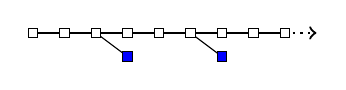
\begin{tikzpicture}[domain=1:10,scale=0.4, every node/.style={scale=0.4}]
					\coordinate (o1) at (1,1);
					\coordinate (o2) at (2,1);
					\coordinate (o3) at (3,1);
					\coordinate (o4) at (4,1);
					\coordinate (o5) at (5,1);
					\coordinate (o6) at (6,1);
					\coordinate (o7) at (7,1);
					\coordinate (o8) at (8,1);
					\coordinate (o9) at (9,1);
					\coordinate (o10) at (10,1);
					\coordinate (n1) at (1,0.25);
					\coordinate (n2) at (2,0.25);
					\coordinate (n3) at (3,0.25);
					\coordinate (n4) at (4,0.25);
					\coordinate (n5) at (5,0.25);
					\coordinate (n6) at (6,0.25);
					\coordinate (n7) at (7,0.25);
					\coordinate (n8) at (8,0.25);
					\coordinate (n9) at (9,0.25);
					\coordinate (n10) at (10,0.25);
					
					\draw[color=black] (o1) to[] (o2) to[] (o3) to[] (o4) to (o5) to (o6) to (o7) to (o8) to (o9);
					\draw[color=black] (o3) to[] (n4);
					\draw[color=black] (o6) to[] (n7);
					\draw[color=black,thick, dotted, ->] (o9) to[] (o10);
					
					\node (rect) at (o1) [fill=white,draw,minimum width=0.3cm,minimum height=0.3cm] {};
					\node (rect) at (o2) [fill=white,draw,minimum width=0.3cm,minimum height=0.3cm] {};
					\node (rect) at (o3) [fill=white,draw,minimum width=0.3cm,minimum height=0.3cm] {};
					\node (rect) at (o4) [fill=white,draw,minimum width=0.3cm,minimum height=0.3cm] {};
					\node (rect) at (o5) [fill=white,draw,minimum width=0.3cm,minimum height=0.3cm] {};
					\node (rect) at (o6) [fill=white,draw,minimum width=0.3cm,minimum height=0.3cm] {};
					\node (rect) at (o7) [fill=white,draw,minimum width=0.3cm,minimum height=0.3cm] {};
					\node (rect) at (o8) [fill=white,draw,minimum width=0.3cm,minimum height=0.3cm] {};
					\node (rect) at (o9) [fill=white,draw,minimum width=0.3cm,minimum height=0.3cm] {};
					
					\node (rect) at (n4) [fill=scheme,draw,minimum width=0.3cm,minimum height=0.3cm] {};
					
					\node (rect) at (n7) [fill=scheme,draw,minimum width=0.3cm,minimum height=0.3cm] {};
					
				\end{tikzpicture}
				
				\\
				&&\\
				Forced fork &
				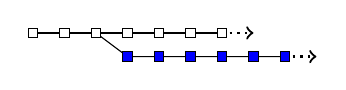
\begin{tikzpicture}[domain=1:10,scale=0.4, every node/.style={scale=0.4}]
					\coordinate (o1) at (1,1);
					\coordinate (o2) at (2,1);
					\coordinate (o3) at (3,1);
					\coordinate (o4) at (4,1);
					\coordinate (o5) at (5,1);
					\coordinate (o6) at (6,1);
					\coordinate (o7) at (7,1);
					\coordinate (o8) at (8,1);
					\coordinate (o9) at (9,1);
					\coordinate (o10) at (10,1);
					\coordinate (n1) at (1,0.25);
					\coordinate (n2) at (2,0.25);
					\coordinate (n3) at (3,0.25);
					\coordinate (n4) at (4,0.25);
					\coordinate (n5) at (5,0.25);
					\coordinate (n6) at (6,0.25);
					\coordinate (n7) at (7,0.25);
					\coordinate (n8) at (8,0.25);
					\coordinate (n9) at (9,0.25);
					\coordinate (n10) at (10,0.25);
					
					\draw[color=black] (o1) to[] (o2) to[] (o3) to[] (o4) to (o5) to (o6) to (o7);
					\draw[color=black] (o3) to[] (n4) to[] (n5) to[] (n6) to[] (n7) to[] (n8) to[] (n9);
					\draw[color=black,thick, dotted, ->] (o7) to[] (o8);
					\draw[color=black,thick, dotted, ->] (n9) to[] (n10);
					
					
					\node (rect) at (o1) [fill=white,draw,minimum width=0.3cm,minimum height=0.3cm] {};
					\node (rect) at (o2) [fill=white,draw,minimum width=0.3cm,minimum height=0.3cm] {};
					\node (rect) at (o3) [fill=white,draw,minimum width=0.3cm,minimum height=0.3cm] {};
					\node (rect) at (o4) [fill=white,draw,minimum width=0.3cm,minimum height=0.3cm] {};
					\node (rect) at (o5) [fill=white,draw,minimum width=0.3cm,minimum height=0.3cm] {};
					\node (rect) at (o6) [fill=white,draw,minimum width=0.3cm,minimum height=0.3cm] {};
					\node (rect) at (o7) [fill=white,draw,minimum width=0.3cm,minimum height=0.3cm] {};
					
					\node (rect) at (n4) [fill=scheme,draw,minimum width=0.3cm,minimum height=0.3cm] {};
					\node (rect) at (n5) [fill=scheme,draw,minimum width=0.3cm,minimum height=0.3cm] {};
					\node (rect) at (n6) [fill=scheme,draw,minimum width=0.3cm,minimum height=0.3cm] {};
					\node (rect) at (n7) [fill=scheme,draw,minimum width=0.3cm,minimum height=0.3cm] {};
					\node (rect) at (n8) [fill=scheme,draw,minimum width=0.3cm,minimum height=0.3cm] {};
					\node (rect) at (n9) [fill=scheme,draw,minimum width=0.3cm,minimum height=0.3cm] {};
				\end{tikzpicture}
				&
				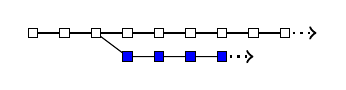
\begin{tikzpicture}[domain=1:10,scale=0.4, every node/.style={scale=0.4}]
					\coordinate (o1) at (1,1);
					\coordinate (o2) at (2,1);
					\coordinate (o3) at (3,1);
					\coordinate (o4) at (4,1);
					\coordinate (o5) at (5,1);
					\coordinate (o6) at (6,1);
					\coordinate (o7) at (7,1);
					\coordinate (o8) at (8,1);
					\coordinate (o9) at (9,1);
					\coordinate (o10) at (10,1);
					\coordinate (n1) at (1,0.25);
					\coordinate (n2) at (2,0.25);
					\coordinate (n3) at (3,0.25);
					\coordinate (n4) at (4,0.25);
					\coordinate (n5) at (5,0.25);
					\coordinate (n6) at (6,0.25);
					\coordinate (n7) at (7,0.25);
					\coordinate (n8) at (8,0.25);
					\coordinate (n9) at (9,0.25);
					\coordinate (n10) at (10,0.25);
					
					\draw[color=black] (o1) to[] (o2) to[] (o3) to[] (o4) to (o5) to (o6) to (o7) to (o8) to (o9);
					\draw[color=black] (o3) to[] (n4) to[] (n5) to[] (n6) to[] (n7);
					\draw[color=black,thick, dotted, ->] (o9) to[] (o10);
					\draw[color=black,thick, dotted, ->] (n7) to[] (n8);
					
					\node (rect) at (o1) [fill=white,draw,minimum width=0.3cm,minimum height=0.3cm] {};
					\node (rect) at (o2) [fill=white,draw,minimum width=0.3cm,minimum height=0.3cm] {};
					\node (rect) at (o3) [fill=white,draw,minimum width=0.3cm,minimum height=0.3cm] {};
					\node (rect) at (o4) [fill=white,draw,minimum width=0.3cm,minimum height=0.3cm] {};
					\node (rect) at (o5) [fill=white,draw,minimum width=0.3cm,minimum height=0.3cm] {};
					\node (rect) at (o6) [fill=white,draw,minimum width=0.3cm,minimum height=0.3cm] {};
					\node (rect) at (o7) [fill=white,draw,minimum width=0.3cm,minimum height=0.3cm] {};
					\node (rect) at (o8) [fill=white,draw,minimum width=0.3cm,minimum height=0.3cm] {};
					\node (rect) at (o9) [fill=white,draw,minimum width=0.3cm,minimum height=0.3cm] {};
					\node (rect) at (n4) [fill=scheme,draw,minimum width=0.3cm,minimum height=0.3cm] {};
					\node (rect) at (n5) [fill=scheme,draw,minimum width=0.3cm,minimum height=0.3cm] {};
					\node (rect) at (n6) [fill=scheme,draw,minimum width=0.3cm,minimum height=0.3cm] {};
					\node (rect) at (n7) [fill=scheme,draw,minimum width=0.3cm,minimum height=0.3cm] {};
				\end{tikzpicture}    
				
				\\[0.2cm] 
				\hline \hline
		\end{tabular}}
	\end{table}
	\newpage
	\subsection*{Exercise 1.1}
	In this example we assumed that a block size increase from 1 MB to 2 MB is proposed. It is easily seen that the new rules are less strict, as nodes implementing this new rule set will accept blocks with a size of up to 2 MB. Nodes under the old rule set, however, will still only accept blocks up to 1 MB. This is a clear example of a hard fork.
	\begin{itemize}
		\item[a)] \textbf{New dominant:} Let us first consider the case, when more computational resources use the new, less strict, rule set. Imagine there is a block with more than 1 MB found (blue block). Miners applying the new rule set will naturally accept this block and continue mining on this chain. Miners under the old rules, on the other hand, will not accept this block and continue mining at the preceding block. In this situation miners applying the new rule set would always accept a longer chain based on the old rule set (white blocks), but as there are more miners using the new rule set, the new chain (blue) will grow faster (at least until the next difficulty adjustment) and thus we will end up with a permanent chain split.
		\item[b)] \textbf{Old dominant:} When more miners implement the old rule set, the opposite is true. The chain with the original, stricter, rule set will grow faster. Thus, whenever a block under the new rules (blue) is found, it will sooner or later be overtaken by the old chain (white). As miners applying the new rule set will also accept this chain, they will fall back on mining at the chain implementing the old rules (white). Thus, there we will not see a chain split. Single orphaned blocks, implementing the new rules, may occur though.
	\end{itemize}

	\subsection*{Exercise 1.2}
	In this example, we assumed that under the new rule set there is a minimal transaction fee required to be included in all transactions in a block. With the new rules being stricter than before, this is an example for a soft fork.
	\begin{itemize}
		\item[a)] \textbf{New dominant:} Imagine there is a block found which only includes transactions that fulfill the new required minimal transaction fee. This block will naturally be accepted by the entire network, as it fulfills both the new and the old rule set. Block under the old rule set, however, will not be accepted by nodes implementing the new rule set. If most of the network hash rate is accepting blocks complying to the new rule set, the blue chain will grow faster and thus we will not end up in a chain split. Single orphaned blocks, implementing the old rules, may occur though.\vspace{1cm}
		\item[b)] \textbf{Old dominant:} If most of the network hashing power is mining blocks under the new rule set, the white chain will grow faster, than the blue one. Thus, after some time the white chain (old rule set) will be longer than the blue chain (new rule set), but as the new rules are more strict, it will not be accepted as the longer chain by miners implementing the new rules. We will thus see a permanent chain split.
	\end{itemize}
	
	\subsection*{Exercise 1.3}
	In the last example we assumed that a Bitcoin Improvement Proposal wants to implement a minimal block size of 0.5 MB and a maximal block size of 2 MB. It is apparent that this would result in a forced fork, as both the old and new rule set include blocks, which are not valid under the other rule set. Thus, we will see a chain split no matter the dominance of the new rule set (a) or the old rule set (b).
	
	\subsection*{Exercise 1.4}
	These additional questions are thought to give you the opportunity to train your understanding of the fork categories. We will not look at the differentiation concerning the allocation of computational resources, as this can be applied analogously from the previous discussion.
	\begin{itemize}
		\item[a)] A reduction in the threshold value so that there are on average two blocks found per ten minutes. This change would imply that the required threshold value for the block header of a new block would be reduced, so that there are on average more blocks found. Thus, under the new rule set, blocks with fewer leading zeros in their block header would be accepted. Blocks fulfilling a lower threshold value (stricter) would still be accepted though. With the new rule set being less restrictive than the old, this is a hard fork.
		\item[b)] This example proposed a change of the block reward from the current 6.25 BTC to 5 BTC. Thus, the new rules are stricter, as they do not accept blocks with a block reward higher than 5 BTC. Here, the footnote gave a key piece of information. Bitcoin miners can generally pay themselves less than the maximal block reward if they find a new block. This is what makes this example a soft fork and not a forced fork.
		%\item[c)] This is a complicated one. The correct solution is, that this is a forced fork, because miners include information on the the number of blocks between difficulty adaptations in their blocks. Thus, there would be a field in the blocks which completely differs from the new to the old rule set. If one ignores this fact, this would be a very interesting case, as the type of fork would depend on how the network hash rate develops. If it increases, the threshold for blocks would be adapted to a stricter level after the 1,008 blocks by the nodes implementing the new rules. The remaining miners would not adapt the threshold until the usual 2,016 blocks are found. Thus this would be a soft fork. On the other hand, if the network hash rate decreases the miners implementing the new rule set would increase the threshold after 1,008 blocks and thus make their rule set less strict. This would therefore result in a hard fork.
	\end{itemize}
	
	\newpage
	\section*{Exercise 2}
	
	This question can be answered by simply looking at the distribution of the two rivaling transaction in the network. Remember, that nodes who have already received one of the two transactions will ignore the other transaction and not forward it to other nodes. As described in the exercise, Eve issues transaction $X$ to node $D$ to pay for a coffee and transaction $Y$ to node $B$. This step is shown again in the left figure. Node $D$ will then proceed and send transaction $X$ to the nodes connected to him ($E$ and $H$). At the same time, node $B$ does the same with transaction $Y$ which she sends to nodes $F$ and $C$. Nodes $E$, $H$, $C$ and $F$ will then proceed in the same manner, checking the received transaction and then forwarding it to their peers. Note that, for example, nodes $E$ and $C$ will each send a different transaction to each other. Both nodes will, however, ignore the second transaction, according to the rules defined.
	
	\begin{figure}[h!]
		\begin{minipage}{0.45\linewidth}
			\centering
			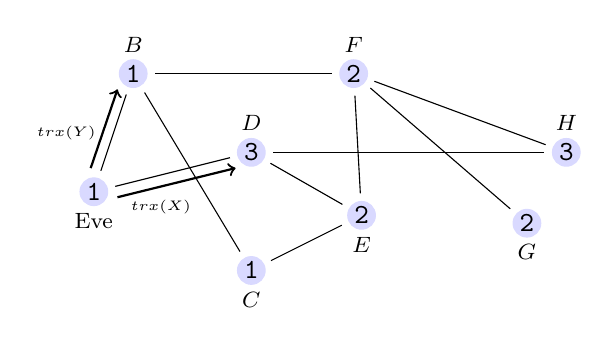
\begin{tikzpicture}[domain=-8:8]
				\coordinate (c1) at (5,0);%Edith
				\coordinate (c2) at (7,-1);%Tony
				\coordinate (c3) at (7,0.5);%Marcia
				\coordinate (c4) at (8.4,-0.3);%Mich\`ele'ss
				\coordinate (c5) at (8.3,1.5);%Brian
				\coordinate (c6) at (11,0.5);%Jake
				\coordinate (c7) at (10.5,-0.4);%Claudia
				\coordinate (c8) at (5.5,1.5);%B
				\coordinate (z1) at (4.65,0.75);%trx(y)
				\coordinate (z2) at (5.85,-0.2);%trx(x)
				\filldraw[color=scheme!15] (c1) circle (5pt) node[color=black]{\texttt{1}} node[below=0.15cm,color=black]{\footnotesize{Eve}};
				\filldraw[color=scheme!15] (c2) circle (5pt) node[color=black]{\texttt{1}} node[below=0.15cm,color=black]{\footnotesize{$C$}};
				\filldraw[color=scheme!15] (c3) circle (5pt) node[color=black]{\texttt{3}} node[above=0.15cm,color=black]{\footnotesize{$D$}};
				\filldraw[color=scheme!15] (c4) circle (5pt) node[color=black]{\texttt{2}} node[below=0.15cm,color=black]{\footnotesize{$E$}};
				\filldraw[color=scheme!15] (c5) circle (5pt) node[color=black]{\texttt{2}} node[above=0.15cm,color=black]{\footnotesize{$F$}};
				\filldraw[color=scheme!15] (c6) circle (5pt) node[color=black]{\texttt{3}} node[above=0.15cm,color=black]{\footnotesize{$H$}};
				\filldraw[color=scheme!15] (c7) circle (5pt) node[color=black]{\texttt{2}} node[below=0.15cm,color=black]{\footnotesize{$G$}};
				\filldraw[color=scheme!15] (c8) circle (5pt) node[color=black]{\texttt{1}} node[above=0.15cm,color=black]{\footnotesize{$B$}};
				
				\draw[shorten >=0.28cm,shorten <=0.28cm] (c1) to[] (c3);
				\draw[shorten >=0.28cm,shorten <=0.28cm] (c1) to[] (c8);
				\draw[shorten >=0.28cm,shorten <=0.28cm] (c2) to[] (c4);
				\draw[shorten >=0.28cm,shorten <=0.28cm] (c2) to[] (c8);
				\draw[shorten >=0.28cm,shorten <=0.28cm] (c3) to[] (c4);
				\draw[shorten >=0.28cm,shorten <=0.28cm] (c3) to[] (c6);
				\draw[shorten >=0.28cm,shorten <=0.28cm] (c4) to[] (c5);
				\draw[shorten >=0.28cm,shorten <=0.28cm] (c5) to[] (c6);
				\draw[shorten >=0.28cm,shorten <=0.28cm] (c5) to[] (c7);
				\draw[shorten >=0.28cm,shorten <=0.28cm] (c5) to[] (c8);
				
				\draw [color = black,->,thick] (4.96,0.30) to (5.3,1.3);
				\node at (z1)[color=black]{\tiny{$trx(Y)$}};
				\draw [color = black,->,thick] (5.3,-0.07) to (6.8,0.3);
				\node at (z2)[color=black]{\tiny{$trx(X)$}};
				
			\end{tikzpicture}
			\small{Initiation of transaction}
		\end{minipage}
		\hfill
		\begin{minipage}{0.45\linewidth}
			\centering
			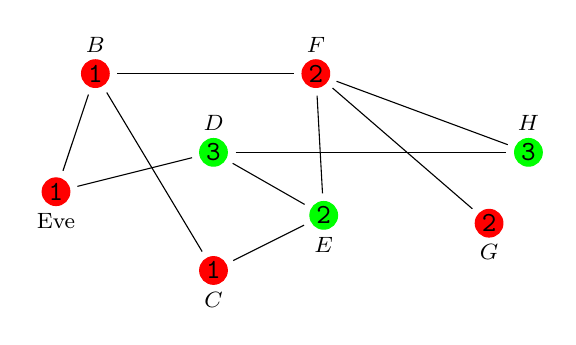
\begin{tikzpicture}[domain=-8:8]
				\coordinate (c1) at (5,0);%Edith
				\coordinate (c2) at (7,-1);%Tony
				\coordinate (c3) at (7,0.5);%Marcia
				\coordinate (c4) at (8.4,-0.3);%Mich\`eles
				\coordinate (c5) at (8.3,1.5);%Brian
				\coordinate (c6) at (11,0.5);%Jake
				\coordinate (c7) at (10.5,-0.4);%Claudia
				\coordinate (c8) at (5.5,1.5);%B
				\coordinate (z1) at (4.65,0.75);%trx(y)
				\coordinate (z2) at (5.85,-0.2);%trx(x)
				
				\draw[shorten >=0.28cm,shorten <=0.28cm] (c1) to[] (c3);
				\draw[shorten >=0.28cm,shorten <=0.28cm] (c1) to[] (c8);
				\draw[shorten >=0.28cm,shorten <=0.28cm] (c2) to[] (c4);
				\draw[shorten >=0.28cm,shorten <=0.28cm] (c2) to[] (c8);
				\draw[shorten >=0.28cm,shorten <=0.28cm] (c3) to[] (c4);
				\draw[shorten >=0.28cm,shorten <=0.28cm] (c3) to[] (c6);
				\draw[shorten >=0.28cm,shorten <=0.28cm] (c4) to[] (c5);
				\draw[shorten >=0.28cm,shorten <=0.28cm] (c5) to[] (c6);
				\draw[shorten >=0.28cm,shorten <=0.28cm] (c5) to[] (c7);
				\draw[shorten >=0.28cm,shorten <=0.28cm] (c5) to[] (c8);
				
				\filldraw[color=red] (c1) circle (5pt) node[color=black]{\texttt{1}} node[below=0.15cm,color=black]{\footnotesize{Eve}};
				\filldraw[color=red] (c2) circle (5pt) node[color=black]{\texttt{1}} node[below=0.15cm,color=black]{\footnotesize{$C$}};
				\filldraw[color=green] (c3) circle (5pt) node[color=black]{\texttt{3}} node[above=0.15cm,color=black]{\footnotesize{$D$}};
				\filldraw[color=green] (c4) circle (5pt) node[color=black]{\texttt{2}} node[below=0.15cm,color=black]{\footnotesize{$E$}};
				\filldraw[color=red] (c5) circle (5pt) node[color=black]{\texttt{2}} node[above=0.15cm,color=black]{\footnotesize{$F$}};
				\filldraw[color=green] (c6) circle (5pt) node[color=black]{\texttt{3}} node[above=0.15cm,color=black]{\footnotesize{$H$}};
				\filldraw[color=red] (c7) circle (5pt) node[color=black]{\texttt{2}} node[below=0.15cm,color=black]{\footnotesize{$G$}};
				\filldraw[color=red] (c8) circle (5pt) node[color=black]{\texttt{1}} node[above=0.15cm,color=black]{\footnotesize{$B$}};
			\end{tikzpicture}
			\small{Distribution of transaction}
		\end{minipage}
	\end{figure}
	
	The network on the right shows which nodes end up including which transaction in their block candidates. The red shaded nodes use $trx(Y)$ and the green ones $trx(X)$. Note in passing, that we were able to present the distribution of the two transactions in such a sequentially ordered manner, because we assumed homogeneous connections between the nodes. In the original Bitcoin network the distribution cannot be divided into such neat sequential steps.\par
	
	To calculate the probability of the double spend attack being successful, we have to calculate the probability of $trx(Y)$ being included in the next block. This is simply done by adding the hash rate of the miners using $trx(Y)$ in their block candidate and dividing by the total hash rate in the network:
	\begin{align*}
		&\text{Hash Power $trx(Y)$:}\quad 1+1+1+2+2=7\\
		&\text{Total Hash Power:}\quad \; \; \: 3+2+3+7=15\\
	\end{align*}
	
	\vspace{-0.9cm}
	Following the calculations above, the probability of success for the double spend attack is $\frac{7}{15} \approx 46.7\% $.
	
	\newpage
	
	\section*{Exercise 3}
	In this exercise we consider the same network structure, but focus on the expected payoff and standard deviation of miner $H$.
	
	\begin{figure}[h!]
		\begin{minipage}{0.45\textwidth}
			\centering
			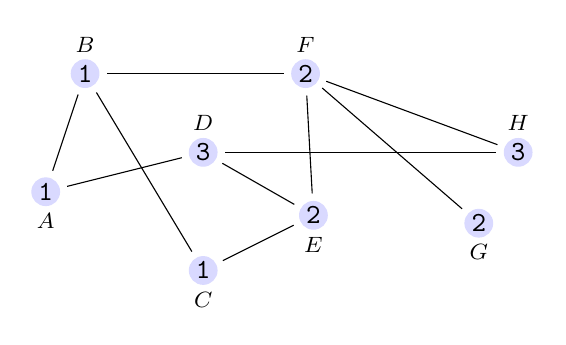
\begin{tikzpicture}[domain=-8:8]
				\coordinate (c1) at (5,0);%Edith
				\coordinate (c2) at (7,-1);%Tony
				\coordinate (c3) at (7,0.5);%Marcia
				\coordinate (c4) at (8.4,-0.3);%Mich\`eles
				\coordinate (c5) at (8.3,1.5);%Brian
				\coordinate (c6) at (11,0.5);%Jake
				\coordinate (c7) at (10.5,-0.4);%Claudia
				\coordinate (c8) at (5.5,1.5);%Tamara
				\filldraw[color=scheme!15] (c1) circle (5pt) node[color=black]{\texttt{1}} node[below=0.15cm,color=black]{\footnotesize{$A$}};
				\filldraw[color=scheme!15] (c2) circle (5pt) node[color=black]{\texttt{1}} node[below=0.15cm,color=black]{\footnotesize{$C$}};
				\filldraw[color=scheme!15] (c3) circle (5pt) node[color=black]{\texttt{3}} node[above=0.15cm,color=black]{\footnotesize{$D$}};
				\filldraw[color=scheme!15] (c4) circle (5pt) node[color=black]{\texttt{2}} node[below=0.15cm,color=black]{\footnotesize{$E$}};
				\filldraw[color=scheme!15] (c5) circle (5pt) node[color=black]{\texttt{2}} node[above=0.15cm,color=black]{\footnotesize{$F$}};
				\filldraw[color=scheme!15] (c6) circle (5pt) node[color=black]{\texttt{3}} node[above=0.15cm,color=black]{\footnotesize{$H$}};
				\filldraw[color=scheme!15] (c7) circle (5pt) node[color=black]{\texttt{2}} node[below=0.15cm,color=black]{\footnotesize{$G$}};
				\filldraw[color=scheme!15] (c8) circle (5pt) node[color=black]{\texttt{1}} node[above=0.15cm,color=black]{\footnotesize{$B$}};
				
				\draw[shorten >=0.28cm,shorten <=0.28cm] (c1) to[] (c3);
				\draw[shorten >=0.28cm,shorten <=0.28cm] (c1) to[] (c8);
				\draw[shorten >=0.28cm,shorten <=0.28cm] (c2) to[] (c4);
				\draw[shorten >=0.28cm,shorten <=0.28cm] (c2) to[] (c8);
				\draw[shorten >=0.28cm,shorten <=0.28cm] (c3) to[] (c4);
				\draw[shorten >=0.28cm,shorten <=0.28cm] (c3) to[] (c6);
				\draw[shorten >=0.28cm,shorten <=0.28cm] (c4) to[] (c5);
				\draw[shorten >=0.28cm,shorten <=0.28cm] (c5) to[] (c6);
				\draw[shorten >=0.28cm,shorten <=0.28cm] (c5) to[] (c7);
				\draw[shorten >=0.28cm,shorten <=0.28cm] (c5) to[] (c8);
			\end{tikzpicture}
		\end{minipage}
		\hfill
		\begin{minipage}{0.45\textwidth}
			\centering
			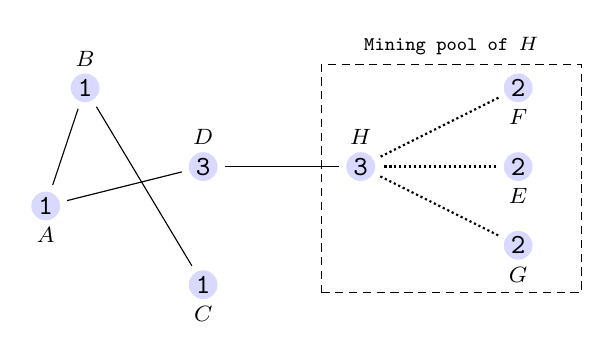
\begin{tikzpicture}[domain=-8:8]
				\coordinate (c1) at (5,0);%A
				\coordinate (c2) at (7,-1);%C
				\coordinate (c3) at (7,0.5);%D
				\coordinate (c4) at (11,0.5);%E
				\coordinate (c5) at (11,1.5);%F
				\coordinate (c6) at (9,0.5);%H
				\coordinate (c7) at (11,-0.5);%G
				\coordinate (c8) at (5.5,1.5);%B
				
				\draw[densely dashed] (8.5,-1.1)--(11.8,-1.1)--(11.8,1.8)--(8.5,1.8)node[midway,above]{\scriptsize{\texttt{Mining pool of $H$}}}--(8.5,-1.1);
				
				\filldraw[color=scheme!15] (c1) circle (5pt) node[color=black]{\texttt{1}} node[below=0.15cm,color=black]{\footnotesize{$A$}};
				\filldraw[color=scheme!15] (c2) circle (5pt) node[color=black]{\texttt{1}} node[below=0.15cm,color=black]{\footnotesize{$C$}};
				\filldraw[color=scheme!15] (c3) circle (5pt) node[color=black]{\texttt{3}} node[above=0.15cm,color=black]{\footnotesize{$D$}};
				\filldraw[color=scheme!15] (c4) circle (5pt) node[color=black]{\texttt{2}} node[below=0.15cm,color=black]{\footnotesize{$E$}};
				\filldraw[color=scheme!15] (c5) circle (5pt) node[color=black]{\texttt{2}} node[below=0.15cm,color=black]{\footnotesize{$F$}};
				\filldraw[color=scheme!15] (c6) circle (5pt) node[color=black]{\texttt{3}} node[above=0.15cm,color=black]{\footnotesize{$H$}};
				\filldraw[color=scheme!15] (c7) circle (5pt) node[color=black]{\texttt{2}} node[below=0.15cm,color=black]{\footnotesize{$G$}};
				\filldraw[color=scheme!15] (c8) circle (5pt) node[color=black]{\texttt{1}} node[above=0.15cm,color=black]{\footnotesize{$B$}};
				
				\draw[shorten >=0.28cm,shorten <=0.28cm] (c1) to[] (c3);
				\draw[shorten >=0.28cm,shorten <=0.28cm] (c1) to[] (c8);
				\draw[shorten >=0.28cm,shorten <=0.28cm] (c2) to[] (c8);
				\draw[shorten >=0.28cm,shorten <=0.28cm] (c3) to[] (c6);
				\draw[shorten >=0.28cm,shorten <=0.28cm,densely dotted,thick] (c4) to[] (c6);
				\draw[shorten >=0.28cm,shorten <=0.28cm,densely dotted,thick] (c5) to[] (c6);
				\draw[shorten >=0.28cm,shorten <=0.28cm,densely dotted,thick] (c6) to[] (c7);
			\end{tikzpicture}
		\end{minipage}
	\end{figure}
	
	\subsection*{Exercise 3.1}
	\begin{itemize}
		\item[a)] To calculate the expected payoff $\mathbb{E}[R]$ of miner $H$ from the next block we simply multiply the possible payoff (6.25 BTC block reward) with the probability that miner $H$ finds the next block. Thus, the expected payoff to miner $H$ is:
		\begin{center}
			$\mathbb{E}[R] = \frac{3}{15} \cdot 6.25 \, \text{BTC} = 1.25 = \mu$
		\end{center}
		\item[b)] Next we calculate the standard deviation $\sigma$ of the expected payoff, which is the square root of the variance of the payoff. The variance is calculated using\\[0.2cm]
		$\sigma^2 = \sum_{x_i}(x_i - \mu)^2 \cdot P(X=x_i) = (6.25-1.25)^{2} \cdot \frac{3}{15} + (0-1.25)^{2} \cdot \frac{12}{15} =  6.25.$\\[0.3cm]
		Thus the standard deviation of the payoff to miner $H$ is $\sigma = \sqrt{6.25} = 2.5$.
	\end{itemize}
	
	\subsection*{Exercise 3.2}
	\begin{itemize}
		\item[a)] The expected payoff $\mathbb{E}[R]$ of miner $H$ in the mining pool is computed very similar to before. However, one has to consider, that she will not receive the full 6.25 BTC payoff if her mining pool finds the next block. Instead she receives a part of the payoff according to her share in the mining pool hash rate.
		\begin{center}
			$\mathbb{E}[R] = \frac{9}{15} \cdot \frac{3}{9} \cdot 6.25 \, \text{BTC} = 1.25 = \mu$
		\end{center}
		Unsurprisingly, her expected payoff stays the same, compared to solo-mining, because the $9$ cancels out. Thus, miner $H$ cannot improve her expected payoff by joining a mining pool. 
		\item[b)] Next, we calculate again the standard deviation $\sigma$ of the expected payoff while considering the share of miner $H$ in the mining pool.
		\begin{align*}
			\sigma^{2} = ((6.25 \cdot \frac{3}{9})-1.25)^{2} \cdot \frac{9}{15} + (0-1.25)^{2} \cdot \frac{6}{15} \approx  1.042
		\end{align*}
		The standard deviation of the payoff to miner $H$ is $\sigma = \sqrt{1.042} \approx 1.021$. This little exercise shows, that miners can decrease the standard deviation of their rewards considerably when joining a mining pool. This will be found desirable by most people, as we generally prefer more regular payments over one-time larger payments.
		\item[c)] Some issues are connected with mining pools that control a large shares of the computational resources in a Blockchain network. First of all, the mining pools could decide to ignore transactions from a specific address, thereby delaying the processing of these transactions (other miners will still include the transactions in their block candidates though). In addition to that, powerful mining pools could try to run so-called 51\%-attacks and overtake the existing longest chain. This could be done to nullify unwanted transactions included in the blocks that are being attacked. Importantly, it is \textbf{never} possible to arbitrarily change transactions (inputs, outputs etc.). We will have a closer look at 51\%-attacks and block races in the next exercise.
	\end{itemize}
	
	\vspace{0.75cm}
	\textbf{Alternative calculation of the standard deviation}\\
	Some of you may have taken another approach to calculate the standard deviations of the expected payoff. Let the random variable $X$ represent if miner $H$ has success (1) or not (0) in finding the next block. Then $X$ follows the binomial distribution, i.e. $X \sim B(n;p)$. In our case $n = 1$ (only one block) and the probability for success is $p=\frac{1}{5}$. Thus, using the equation for the standard deviation of a random variable following the binomial distribution we receive
	\begin{align*}
		\sigma^{2}(x) &= \overbrace{n}^{=1} \cdot p \cdot (1-p)\\
		\intertext{and}
		\sigma(x) &= \sqrt{\frac{1}{5} \cdot \frac{4}{5}} = \frac{2}{5}
	\end{align*}
	Multiplying the result with the payoff in case of success gives $\sigma = \frac{2}{5} \cdot 6.25 = 2.5$ and thus the same result as in Exercise 3.1.
	
	\newpage
	\section*{Exercise 4}
	\subsection*{Exercise 4.1}
	As described in the exercise, Michèle and Tony have found a block at the same time, but since then, two blocks were added based on Michèle's block. Tony is very unhappy about this, as he has lost the block reward included in his block because of this. Therefore, he could try to save his initial block reward by finding three consecutive blocks and overtaking the chain with Michèle's block. The figure below depicts the situation:
	\begin{figure}[h!]
		\centering
		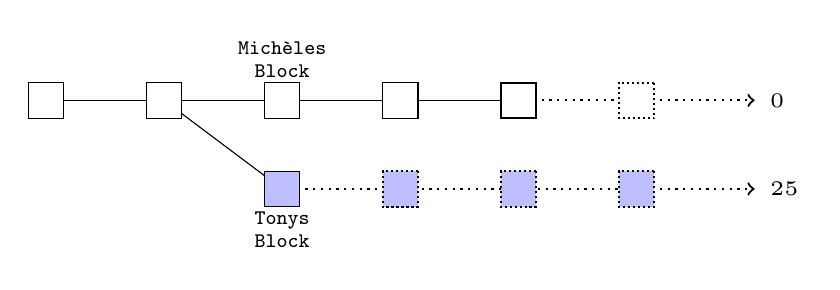
\begin{tikzpicture}[domain=1:10,scale=1.5, every node/.style={scale=1.5}]
			\coordinate (o1) at (1,1);
			\coordinate (o2) at (2,1);
			\coordinate (o3) at (3,1);
			\coordinate (o4) at (4,1);
			\coordinate (o5) at (5,1);
			\coordinate (o6) at (6,1);
			\coordinate (o7) at (7,1);
			\coordinate (o8) at (8,1);
			\coordinate (o9) at (9,1);
			\coordinate (o10) at (10,1);
			\coordinate (n1) at (1,0.25);
			\coordinate (n2) at (2,0.250);
			\coordinate (n3) at (3,0.250);
			\coordinate (n4) at (4,0.250);
			\coordinate (n5) at (5,0.250);
			\coordinate (n6) at (6,0.250);
			\coordinate (n7) at (7,0.250);
			\coordinate (n8) at (8,0.250);
			\coordinate (n9) at (9,0.250);
			\coordinate (n10) at (10,0.250);
			
			\draw[] (o1) -- (o2) -- (o3) -- (o4) -- (o5);
			\draw[] (o2) -- (n3); 
			\draw[dotted, thick] (n3) -- (n4) -- (n5) -- (n6);
			\draw[dotted, thick] (o5) -- (o6);
			\draw[color=black,thick, dotted, ->] (o6) to[] (o7) node[right]{\tiny{$0$}};
			\draw[color=black,thick, dotted, ->] (n6) to[] (n7) node[right]{\tiny{$25$}};
			
			\node (rect) at (o1) [fill=white,draw,minimum width=0.3cm,minimum height=0.3cm] {};
			\node (rect) at (o2) [fill=white,draw,minimum width=0.3cm,minimum height=0.3cm] {};
			\node (rect) at (o3) [fill=white,draw,minimum width=0.3cm,minimum height=0.3cm] {};
			\node (rect) at (o4) [fill=white,draw,minimum width=0.3cm,minimum height=0.3cm] {};
			\node at (o3) [above=0.1cm]{\tiny{\texttt{Block}}};
			\node at (o3) [above=0.4cm]{\tiny{\texttt{Mich\`eles}}};
			\node at (n3) [below=0.4cm]{\tiny{\texttt{Block}}};
			\node at (n3) [below=0.1cm]{\tiny{\texttt{Tonys}}};
			\node (rect) at (o5) [fill=white,thick,draw,minimum width=0.3cm,minimum height=0.3cm] {};
			\node (rect) at (o6) [thick, densely dotted, fill=white,draw,minimum width=0.3cm,minimum height=0.3cm] {};
			\node (rect) at (n3) [fill=scheme!25,draw,minimum width=0.3cm,minimum height=0.3cm] {};
			\node (rect) at (n4) [thick,fill=scheme!25,draw,minimum width=0.3cm,minimum height=0.3cm,densely dotted] {};
			\node (rect) at (n5) [thick,fill=scheme!25,draw,minimum width=0.3cm,minimum height=0.3cm,densely dotted] {};
			\node (rect) at (n6) [thick, densely dotted, fill=scheme!25,draw,minimum width=0.3cm,minimum height=0.3cm] {};
		\end{tikzpicture}
	\end{figure}
	The exercise then asked to compute the relative hashing power $\frac{h}{H}$ of Tony with which he would be indifferent between trying to save his initial block reward (option 1) and continuing at the current state of Michèles chain (option 2). We therefore have to calculate the expected payoff for both options, set them equal and solve for the relative hash rate.
	\begin{align*}
		\overbrace{3\left[\frac{h}{H}\right]R}^{\text{Option 2}}&=\overbrace{\left[\frac{h}{H}\right]^3 4R}^{\text{Option 1}}\\
		3&= \left[\frac{h}{H}\right]^2 4\\
		\sqrt[]{\frac{3}{4}}=\frac{\sqrt[]{3}}{2}&=\frac{h}{H}\approx 0.866
	\end{align*}
	In order to overtake the currently longest chain, based on Michèle's block, Tony would have to find three consecutive blocks. The probability for this is $\left[\frac{h}{H}\right]^3$ and the payoff would be three block rewards for the three blocks found, plus the block reward included in the original block Tony is trying to save. Option 2 would simply give him three times the expected payoff, as used in Exercise 3. Solving for the relative hash rate leads to the result, that Tony would have to control $86.6\%$ of the hashing power in the entire network. The table below illustrates what the required relative hash rate would be to make Tony indifferent for different distances to the chain with Michèle's block.
	\begin{table}[h!]
		\centering
		\resizebox{11cm}{!} {
			\begin{tabular}{c c c c c c c c c c c}
				\hline \hline Distance & 1 & 2 & 3 & 4 & 5 & 6 & 7 & 8 & 9 & 10 \\
				$\frac{h}{H}$ & .667 & .866 & .928 & .955 & .970 & .980 & .983 & .987 & .989 & .991\\
				\hline \hline
			\end{tabular}
		}
	\end{table}
	
	\subsection*{Exercise 4.2}
	Next, we slightly changed the story and assumed that there is only one additional block in Michèle's chain. In addition to that we assumed that there were unusually high transaction fees included in the two initially found blocks by Tony and Michèle. We denoted these high transaction fees with $f > 0$. All remaining blocks only include the usual transaction fees, which we assumed to be zero for simplicity. 
	\begin{figure}[h!]
		\centering
		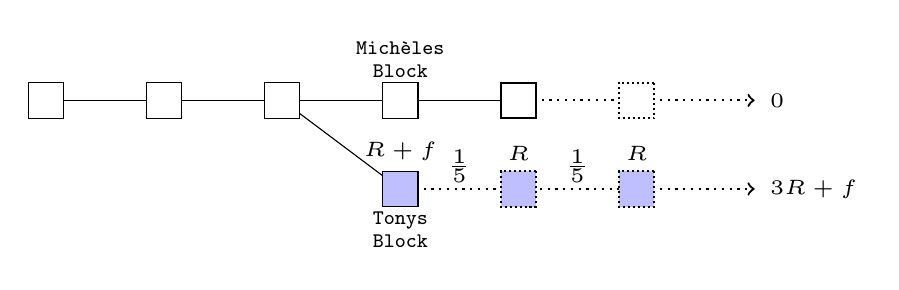
\begin{tikzpicture}[domain=1:10,scale=1.5, every node/.style={scale=1.5}]
			\coordinate (o1) at (1,1);
			\coordinate (o2) at (2,1);
			\coordinate (o3) at (3,1);
			\coordinate (o4) at (4,1);
			\coordinate (o5) at (5,1);
			\coordinate (o6) at (6,1);
			\coordinate (o7) at (7,1);
			\coordinate (o8) at (8,1);
			\coordinate (o9) at (9,1);
			\coordinate (o10) at (10,1);
			\coordinate (n1) at (1,0.25);
			\coordinate (n2) at (2,0.250);
			\coordinate (n3) at (3,0.250);
			\coordinate (n4) at (4,0.250);
			\coordinate (n5) at (5,0.250);
			\coordinate (n6) at (6,0.250);
			\coordinate (n7) at (7,0.250);
			\coordinate (n8) at (8,0.250);
			\coordinate (n9) at (9,0.250);
			\coordinate (n10) at (10,0.250);
			
			\draw[] (o1) -- (o2) -- (o3) -- (o4) -- (o5) ;
			\draw[] (o3) -- (n4); 
			\draw[dotted, thick] (n4) -- (n5) node[midway, yshift=0.19cm]{\tiny{$\frac{1}{5}$}} -- (n6) node[midway, yshift=0.19cm]{\tiny{$\frac{1}{5}$}} ;
			\draw[dotted, thick] (o5) -- (o6);
			\draw[color=black,thick, dotted, ->] (o6) to[] (o7) node[right]{\tiny{$0$}};
			\draw[color=black,thick, dotted, ->] (n6) to[] (n7) node[right]{\tiny{\(3R+f\)}};
			
			\node (rect) at (o1) [fill=white,draw,minimum width=0.3cm,minimum height=0.3cm] {};
			\node (rect) at (o2) [fill=white,draw,minimum width=0.3cm,minimum height=0.3cm] {};
			\node (rect) at (o3) [fill=white,draw,minimum width=0.3cm,minimum height=0.3cm] {};
			\node (rect) at (o4) [fill=white,draw,minimum width=0.3cm,minimum height=0.3cm] {};
			\node at (o4) [above=0.1cm]{\tiny{\texttt{Block}}};
			\node at (o4) [above=0.4cm]{\tiny{\texttt{Mich\`eles}}};
			\node at (n4) [below=0.4cm]{\tiny{\texttt{Block}}};
			\node at (n4) [below=0.1cm]{\tiny{\texttt{Tonys}}};
			
			\node at (n4) [above=0.175cm,color=black]{\tiny{\(R+f\)}};
			\node at (n5) [above=0.175cm,color=black]{\tiny{\(R\)}};
			\node at (n6) [above=0.175cm,color=black]{\tiny{\(R\)}};
			
			\node (rect) at (o5) [fill=white,draw,thick,minimum width=0.3cm,minimum height=0.3cm] {};
			\node (rect) at (o6) [thick, densely dotted, fill=white,draw,minimum width=0.3cm,minimum height=0.3cm] {};
			\node (rect) at (n4) [fill=scheme!25,draw,minimum width=0.3cm,minimum height=0.3cm] {};
			\node (rect) at (n5) [thick,fill=scheme!25,draw,minimum width=0.3cm,minimum height=0.3cm,densely dotted] {};
			\node (rect) at (n6) [thick, densely dotted, fill=scheme!25,draw,minimum width=0.3cm,minimum height=0.3cm] {};
		\end{tikzpicture}
	\end{figure}
	In this exercise we asked you to formulate again the equation which sets equal the expected payoffs of Tony's options, but then solve for the transaction fee $f$. This to find the resulting relation between $f$ and $R$ if we assume the relative hashing power of Tony to be 20\%, i.e. $\frac{h}{H} = \frac{1}{5}$.
	\begin{align*}
		\overbrace{2 \left[\frac{h}{H}\right]R}^{\text{Option 2}}&=\overbrace{\left[\frac{h}{H}\right]^2 (3R+f)}^{\text{Option 1}}\\
		2R&=\left[\frac{h}{H}\right] (3R+f)\\
		2R\left[\frac{5}{1}\right]-3R&=f\\
		7R&=f
	\end{align*}
	This time, Tony only has to find two consecutive blocks to overtake the currently longest chain, which is reflected in the first line above. Note that he would therefore receive two block rewards for these blocks, plus the original block reward and the transaction fee, if he succeeds ($3R + f$). Solving for the transaction fees $f$ gives us the result, that the transaction fee would have to amount to seven times the current block reward to make Tony indifferent between the two options if he controls one-fifth of the network hash rate.
	\newpage
	Solving Exercise 4.2 you might have asked yourself if these seemingly theoretical calculations have any relevance in practice. In fact, in 2016 there was an incident where someone included $\sim 291$ BTC as transaction fees in their transaction\footnote{cc455ae816e6cdafdb58d54e35d4f46d860047458eacf1c7405dc634631c570d}. This, of course, drastically increased the transaction fees included in the block (number 409008) comparing to the $0.4$ BTC transaction fees included in the next block. Luckily, the important difference to our example story was, that there were not coincidentally two blocks found at the same time both including this unusual transaction.\par 
	
	The interested reader could now wonder, what relative hashing power a miner would have needed at that time to be indifferent between the two options Tony faced in Exercise 4.2. Assuming only one block was added to the chain with Michèle's block and considering that the block reward was 25 BTC at that time we can calculate
	\begin{align*}
		\overbrace{\left[\frac{h}{H}\right]R+\left[\frac{h}{H}\right]R}^{\text{Option 1}}&=\overbrace{\left[\frac{h}{H}\right]^2 (3R+f)}^{\text{Option 2}}\\
		2R&=\left[\frac{h}{H}\right] (3R+f)\\
		\frac{2R}{(3R+f)}&=\left[\frac{h}{H}\right]\\
		\frac{50}{(75+291)}=\frac{50}{366}&=\left[\frac{h}{H}\right] \approx 0.1366\\
	\end{align*}
	which is a relative hash rate big mining pools often surpass. To avoid misunderstandings, be reminded that in order to face such a trade off, two miners (or mining pools) would have to each find a block at the same time, both including the unusually high transaction fees. However, with the decreasing block reward and the increasing popularity (and thus increasing transaction fees) of Bitcoin, events like this become more and more probable.
\end{document}
